% Use the lineno option to display guide line numbers if required.
\documentclass[9pt,twocolumn,twoside,lineno]{pnas-new}

\usepackage{listings}

% Automatic formatting of SI units
\usepackage[binary-units]{siunitx}

% Set options for code listings
\lstset{language=C++}

% Visible TODO notes
\newcommand{\todo}[1]{\textbf{\textsc{\textcolor{red}{(TODO: #1)}}}}

\templatetype{pnasresearcharticle} % Choose template 
% {pnasresearcharticle} = Template for a two-column research article
% {pnasmathematics} %= Template for a one-column mathematics article
% {pnasinvited} %= Template for a PNAS invited submission

\title{Large-scale brain simulations on the desktop using procedural connectivity}

% Use letters for affiliations, numbers to show equal authorship (if applicable) and to indicate the corresponding author
\author[a,1]{James C Knight}
\author[a]{Thomas Nowotny} 

\affil[a]{Centre for Computational Neuroscience and Robotics, School of Engineering and Informatics, University of Sussex, Brighton, United Kingdom}

% Please give the surname of the lead author for the running footer
\leadauthor{Knight} 

% Please add here a significance statement to explain the relevance of your work
\significancestatement{Authors must submit a 120-word maximum statement about the significance of their research paper written at a level understandable to an undergraduate educated scientist outside their field of speciality. The primary goal of the Significance Statement is to explain the relevance of the work in broad context to a broad readership. The Significance Statement appears in the paper itself and is required for all research papers.}

% Please include corresponding author, author contribution and author declaration information
\authorcontributions{J.K. and T.N. wrote the paper.
T.N. is the original developer of GeNN.
J.K. is currently the primary GeNN developer and was responsible for extending the code generation approach to the procedural simulation of synaptic connectivity.
J.K. performed the experiments and the analysis of the results that are presented in this work.}

\authordeclaration{The authors declare no conflict of interest.}
\correspondingauthor{\textsuperscript{1}To whom correspondence should be addressed. E-mail: J.C.Knight\@sussex.ac.uk}

% Keywords are not mandatory, but authors are strongly encouraged to provide them. If provided, please include two to five keywords, separated by the pipe symbol, e.g:
\keywords{spiking neural networks $|$ GPU $|$ high-performance computing $|$ brain simulation} 

\begin{abstract}
Large-scale simulations of spiking neural networks have become important tools in helping us improve the dynamics and, ultimately, the function of the brain.
However, even small mammals such as mice have around \num{1E12} synaptic connections~\citep{Herculano-Houzel2010}, the strengths of which are typically modelled as individual floating point values.
If single precision floating point were used to store these values, several terabytes of memory would be required.
As such memory requirements are beyond what is plausible for a single machine, simulations of large-scale spiking neural network currently are typically simulated on large distributed systems.
Large parts of such models are typically described by simple algorithms which describe connectivity and the strength of synaptic connections.
In this work, we describe our extensions to GeNN~\citep{Yavuz2016} -- our GPU-based spiking neural network simulator -- to enable it to `procedurally' generate connectivity and synaptic weights as spikes are received rather than retrieving them in memory.
We find that high-end GPUs are well-suited to this approach as they provide a large amount of raw computational power which is often under-utilised when simulating spiking neural networks due to the limited memory bandwidth available to each parallel computing element.
To demonstrate the value of this approach, we present the results of simulations of a recent model of the Macaque visual cortex consisting of \num{4.13E6} neurons and \num{24.2E9} synapses on a single GPU and show that the results are correct and the simulation runs faster than previous simulations which ran on over 1000 supercomputer nodes.

\end{abstract}

\dates{This manuscript was compiled on \today}
\doi{\url{www.pnas.org/cgi/doi/10.1073/pnas.XXXXXXXXXX}}

\begin{document}

\maketitle
\thispagestyle{firststyle}
\ifthenelse{\boolean{shortarticle}}{\ifthenelse{\boolean{singlecolumn}}{\abscontentformatted}{\abscontent}}{}

\dropcap{W}hile the brain of a mouse has around \num{70E6} neurons, their numbers are dwarved by the \num{1E12} synapses which connect them.
%While simulating synaptic plasticity -- the family of mechanisms believed to be %responsible for learning -- represents a further challenge, in a large-scale model, it is unlikely that learning would be enabled on \emph{all} synapses so efficiently simulating the remaining static synapses is a key challenge for large-scale brain simulation.\todo{has this been at all quantified in mice?}
Computationally, simulating spikes propagating through synapses involves reading a `row' of synapses connecting a spiking presynaptic neuron to its postsynaptic partners and adding the `weight' of each synapse in the row to a `bin' containing the postsynatic neuron's input for a simulation timestep.
%Because typical EPSP shaping functions are linear, they can then be subsequently applied to the `histogram' resulting from this process.~\todo{presumably someone first had this intuition so cite}.

Because of the high memory requirements of large-scale brain models, they are typically simulated on large distributed systems using software such as NEST~\citep{Gewaltig2007} or NEURON~\citep{carnevale2006neuron}.
By careful design, such simulators can maintain a constant memory requirements for each node can kept constant even when a simulation is distributed across thousands of nodes~\citep{Jordan2018}.
However, such systems are large, expensive and consume large amounts of power meaning that they are typically shared between many researchers from many institutions.

Neuromorphic systems~\citep{Frenkel2018,Frenkel2019,Furber2014,Merolla2014,Qiao2015,Schemmel2017} take inspiration from the brain and have been developed specifically for simulating spiking neural networks.
One particular relevant feature of the brain is that its memory elements -- the synapses -- are located throughout the system rather than being centrally located.
In neuromorphic systems, this often translates to a large proportion of each chip being dedicated to memory.
However, while such on-chip memory is fast, it can only be fabricated at relatively low density meaning that many of these systems economize -- either by reducing the maximum number of synapses per neuron to as few as \num{256} or by reducing the precision of the synaptic weights to \num{6}~\citep{Schemmel2017}, \num{4}~\citep{Frenkel2018} or even \SI{1}{\bit}~\citep{Merolla2014,Frenkel2019}.
While such strategies allow some classes of spiking neural networks to be simulated very efficiently, in the context of large-scale brain simulation, reducing the degree of connectivity to fit within the constraints of such a system inevitably changes its dynamics~\citep{VanAlbada2015}.
Unlike the majority of other other neuromorphic systems, SpiNNaker~\citep{Furber2014} is entirely programmable and combines a large amount of on-chip meory with external memories, distributed across the system for the storage of synaptic connectivity.
SpiNNaker's external memory bandwidth, on-chip memory capacity and the computational power of each core are all tailored to large-scale brain simulation meaning that the output bins of the synapse processing algorithm can fit in on-chip memory and there is enough external memory bandwidth to fetch synaptic rows fast enough for real-time simulation of large-scale models~\citep{Rhodes2019}.
\todo{good argument against SpiNNaker}
%However, a physically large system is required for even moderately-sized simulations (9 boards for a simulation with around \num{10E3} neurons and \num{300E6} synapses~\citep{Rhodes2019})
%A next generation SpiNNaker system is currently under development~\citep{Mayr2019} and, by employing a newer fabrication technology (\SI{22}{\nano\meter} rather than \SI{130}{\nano\meter}), a single chip of the new system will offer equivalent performance to 48 of the current chips.
%Nonetheless, large-scale brain simulations will still require a large multi-chip system.

GPU architectures have relatively small amounts of on-chip memory and, instead, dedicate the majority of their silicon area to arithmetic logic units~(ALUs).
GPUs use dedictated hardware to rapidly switch between tasks meaning that, as long as there is sufficient computation to be performed, the latency of accessing external memory can be `hidden' behind computation.
For example, each CUDA core of a modern GPU needs to perform approximately 10 arithmetic operations per byte of data accessed from memory in order to successfully hide the memory latency.
However, processing a synapse is likely to require accessing approximately \SI{8}{\byte} of memory and performing many fewer than 80 instructions, making this operating highly memory bound.
Nonetheless, in our previous work~\citep{Knight2018} we showed that, as GPUs have significantly higher total memory bandwidth than even the most expensive CPU, moderately sized models of around \num{10E3} neurons and \num{1E9} synapses can be simulated on a single GPU with competitive speed and energy requirements.
Nonetheless, individual GPUs do not have enough memory to simulate truly large-scale brain models and, although small numbers of GPUs can be connected together using the high-speed NVLink~\todo{cite} interconnect, beyond this scaling will be dictated by the same communication overheads as other distributed systems.

In this work we present an approach which converts large-scale brain simulation from a problem which is memory-bound on a GPU to one where the large amount of computational power available on a GPU can be used to reduce the memory and memory bandwidth requirements and make large-scale brain simulations on a single workstation possible.

\section*{Results}
In the following subsections we will first present two novel features of our GeNN simulator~\citep{Yavuz2016} which allow it be used for simulating large-scale models on a single GPU.
Finally, we will demonstrate the power of both features by simulating a recent model of the Macaque visual cortex~\citep{Schmidt2018} consisting of \num{4.13E6} neurons and \num{24.2E9} synapses on a single GPU and demonstratint that, not only are the results correct, but the simulation runs faster than simulations previously run on a supercomputer system.


\subsection*{Procedural connectivity}
Our GeNN simulator~\citep{Yavuz2016} uses code generation to convert neuron and synapse models -- described using `snippets' of C-like code -- into CUDA code for GPU simulation.
We previously extended GeNN to allow the same approach to be applied to generating efficient, parallel model initialisation code from code snippets describing the algorithms to use for initialising individual state variables and synaptic connectivity~\citep{Knight2018}.
Parallelising initialisation in this manner sped up model initialisation by around $20\times$ on a desktop PC, but also indicates just how well-suited these initialisation algorithms are to GPU implementation.
In fact, it seems somewhat illogical to run these algorithms once only to fill the limited memory of the GPU with data and subsequently read it back throughout the simulation at the expense of equally limited memory bandwidth.
Instead, what if we used some of the 

\begin{figure*}
    \centering
    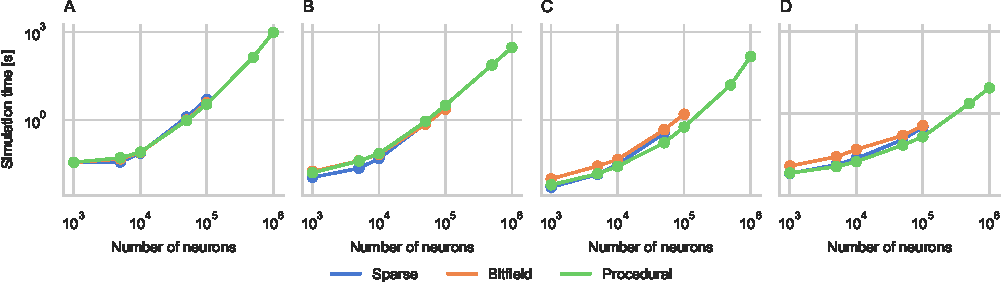
\includegraphics{figures/performance_scaling}
    \caption{Performance scaling on a range of modern GPUs. \textbf{A} The best performing approach at each scale.
    \textbf{B} Raw performance of each approach.}
    \label{fig:performance_scaling}
\end{figure*}

To demonstrate the performance and scalability of this new approach, we ran several simulations of a network, initially designed as a medium for experimentation into signal propagation through cortical networks~\citep{Vogels2005}, but subsequently  widely used as a scalable benchmark~\citep{Brette2007}.
The network consists of \num{10000} integrate-and-fire neurons, split between an excitatory population of \num{8000} cells and an inhibitory population of \num{2000} cells.

\begin{figure*}
    \centering
    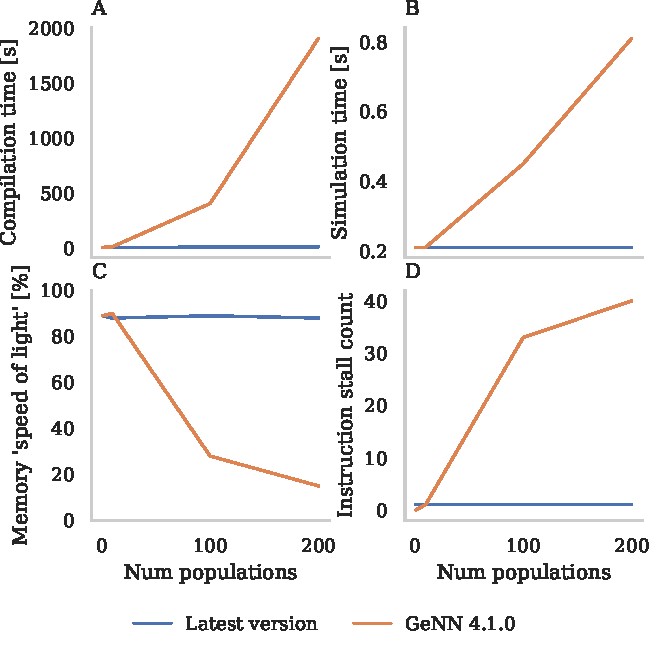
\includegraphics{figures/merging_scaling}
    \caption{Performance of a simulation of \num{1000000} LIF neurons driven by a gaussian input current, partitioned into varying numbers of populations. 
    \textbf{A} Compilation time using GCC 7.5.0.
    \textbf{B} Simulation time for an \SI{1}{\second} simulation.
    \textbf{C} Memory throughput reported by NVIDIA Nsight compute profiler 'Speed of light' metric.
    \textbf{D} Number of 'No instruction' stalls reported by NVIDIA Nsight compute profiler.}
    \label{fig:merging_scaling}
\end{figure*}

\subsection*{Kernel merging}
While the procedural connectivity approach presented in the previous section allows us to simulate models which would otherwise not fit within the memory of a single GPU, there are additional problems when using code generation to generate simulation code for models with large numbers of neuron and synapse populations.

GeNN and -- to the best of our knowledge~\citep{Blundell2018} -- all other SNN simulators which use code generation to generate all of their simulation code (rather than, for example NESTML~\citep{Plotnikov2016}, which uses code generation to generate neuron simulation code) generate seperate pieces of code to simulate each population of neurons and synapses.
This approach allows optimizations such as the hard-coding of constant parameters to be easily performed and, although generating code for models with many populations will result in large code size, C++ CPU code  can be easily divided between multiple modules and compiled in parallel, minimizing the effect on build time.
However, GPUs can only run a small number of kernels -- which are equivalent to modules in this context --  simultaneously (128 on the latest NVIDIA GPUs~\todo{cite}).
Therefore, in GeNN, multiple neuron populations are simulated within each kernel resulting in code such as the following example which illustrates how 3 populations of 1000 neurons could be simulated in a single kernel:

\begin{lstlisting}
void updateNeurons()
{
  if(thread < 1000) {
    // Update neuron population A
  }
  else if(thread >= 1000 && thread < 2000) {
    // Update neuron population B
  }
  else if(thread >= 2000 && thread < 3000) {
    // Update neuron population C
  }
}

\end{lstlisting}

This works well for models with small numbers of populations but, as Fig.~\ref{fig:merging_scaling}A illustrates, compilation time increases super-linearly with the number of populations (i.e. the size of the neuron kernel) -- quickly becoming impractical.
Additionally, and even more critically, Fig.~\ref{fig:merging_scaling}B shows that simulations of the same model, artificially divided into more populations, run much slower.
Each thread in this model reads \SI{32}{\byte} of data and, as we discussed previously, hiding the latency of these memory accesses would require approximately 320 arithmetic operations.
Sampling from the uniform distribution and updating a LIF neuron requires many fewer operations than this so we would expect this kernel to be memory bound.
Fig.~\ref{fig:merging_scaling}C -- obtained using data from the NVIDIA Nsight compute profiler~\todo{cite} -- shows that this to be true with the memory system being around \SI{90}{\percent} utilised for small numbers of populations.
However, if the model is partitioned into large numbers of populations, the kernel stops being able to efficiently use the memory.
Investigating further using the profiler showed that this drop in performance was accompanied by a large number of ``No instruction'' stalls (events preventing the GPU from doing any work during a given clock cycle) as illustrated in Fig.~\ref{fig:merging_scaling}D.

\begin{lstlisting}
struct NeuronUpdateGroup
{
  unsigned int numNeurons;
  float* V; 
};

NeuronUpdateGroup neuronUpdateGroup
{
  {1000, d_VA},
  {1000, d_VB},
  {1000, d_VC}
};

void updateNeurons()
{
  if(thread < 3000) {
    // Determine which population thread
    // should be processing and update using 
    // variables in neuronUpdateGroup
  }
}
\end{lstlisting}

\begin{figure*}
    \centering
    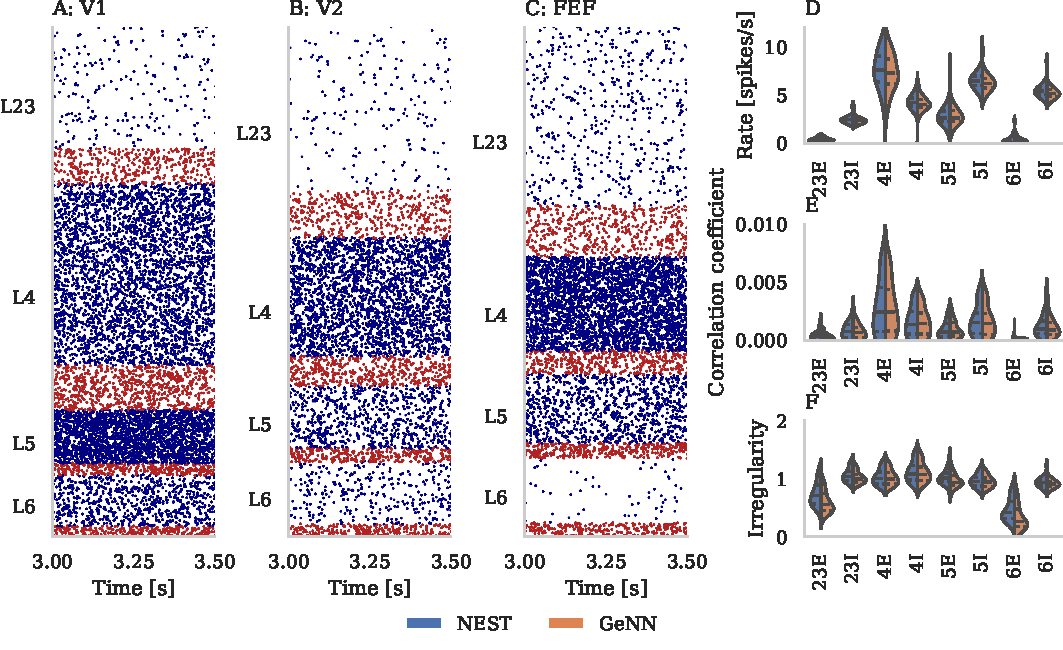
\includegraphics{figures/multi_area}
    \caption{Results of full-scale multi-area model simulation. 
    \textbf{A-C} Raster plots of spiking activity of \SI{3}{\percent} of the neurons in area V1~\textbf{A}, V2~\textbf{B}, and FEF~\textbf{C}. 
    Blue: excitatory neurons, red: inhibitory neurons.
    \textbf{D-F} Spiking statistics for each population across all 32 areas simulated using GeNN and NEST shown as split violin plots.
    Solid lines: medians, Dashed lines: Interquartile range~(IQR).
    \textbf{D} Population-averaged firing rates.
    \textbf{E} Average pairwise correlation coefficients ofspiking activity. 
    \textbf{F} Irregularity measured by revised local variation LvR~\citep{Shinomoto2009} averaged across neurons.}
    \label{fig:multi_area}
\end{figure*}

\subsection*{The multi-area model}
Due to lack of computing power and sufficiently detailed connectivity data, previous models of the cortex have either focussed on modelling individual local microcircuits at the level of individual cells~\citep{Izhikevich2008,Potjans2012} or modelling multiple connected areas at a higher level of abstraction where entire ensembles of neurons are described by a small number of differential equations~\todo{find citation}.
However, data from several species~\todo{find citation} has shown that cortical activity has distinct features at both the global and local levels which can only be captured by modelling interconnected microcircuits at the level of individual cells.
The multi-area model~\citep{Schmidt2018a,Schmidt2018} does just this -- using scaled versions of a previous 4 layer microcircuit model~\citep{Potjans2012} to implement \SI{1}{\milli\meter\squared} `patches' for each of 32 areas of the macaque cortex involved in visual processing.
The 32 areas are connected together with connectivity based on inter-area axon tracing data from the CoCoMac~\citep{Bakker2012} database, further refined using additional anatomical data~\citep{Markov2014} and heuristics~\citep{Ercsey-Ravasz2013} to obtain estimates for the number of synapses connecting pairs of areas.
Synapses between areas are then distributed between the populations which make up each area 

By using a supercomputer to simulate a model based on the latest connectivity data and The multi-scale model of the macaque visual cortex~\citep{Schmidt2018} developed by 


\section*{Discussion}
\begin{itemize}
    \item Further scaling - memory only required for neuron parameters
    \item Learning
    \item Hardware for procedural connectivity?
\end{itemize}


\matmethods{Please describe your materials and methods here. This can be more than one paragraph, and may contain subsections and equations as required. Authors should include a statement in the methods section describing how readers will be able to access the data in the paper. 
\begin{itemize}
    \item LIF neuron
    \item Exponential static synapses
    \item Connectivity
    \item Parameter values for scaling and merging experiments
\end{itemize}
\subsection*{Neuron models}
Example text for subsection.
}

\showmatmethods{} % Display the Materials and Methods section

\acknow{Please include your acknowledgments here, set in a single paragraph. Please do not include any acknowledgments in the Supporting Information, or anywhere else in the manuscript.}

\showacknow{} % Display the acknowledgments section

% Bibliography
\bibliography{procedural}

\end{document}
